\documentclass{standalone}
\usepackage{tikz}
\usetikzlibrary{arrows.meta, positioning}

\begin{document}
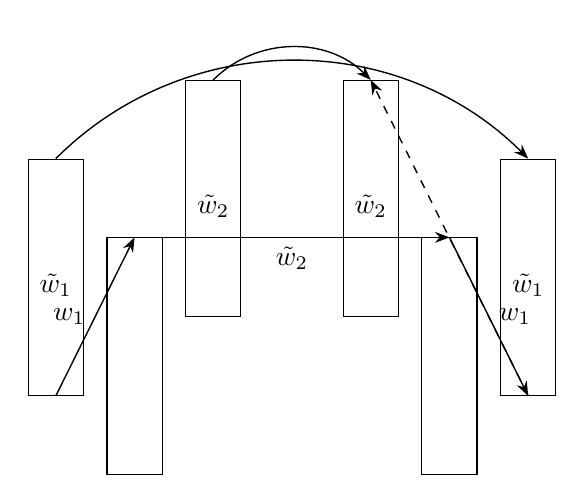
\begin{tikzpicture}[scale=1.0]
  \tikzset{
    rect node/.style={draw, minimum width=0.7cm, minimum height=3cm},
    arrow style/.style={-{Stealth[scale=1]}, line width=0.5pt},
  }

  % Nodes
  \node[rect node] (A1) at (0,0) {};
  \node[rect node] (A2) at (6,0) {};
  \node[rect node] (B1) at (2,1) {};
  \node[rect node] (B2) at (4,1) {};
  \node[rect node] (C1) at (1,-1) {};
  \node[rect node] (C2) at (5,-1) {};

  % Edges
  \draw[arrow style] (A1.south) -- node[midway, left] {$w_1$} (C1.north);
  \draw[arrow style] (C1.north) -- node[midway, below] {$\tilde{w}_2$} (C2.north);
  \draw[arrow style] (C2.north) -- node[midway, right] {$w_1$} (A2.south);
  \draw[arrow style, dashed] (A2.south) -- (B2.north);
  \draw[arrow style] (A1.north) to[bend left=45] node[midway, above] {} (A2.north);
  \draw[arrow style] (B1.north) to[bend left=45] node[midway, above] {} (B2.north);

  % Labels
  \node at (0,-0.1) {$\tilde{w}_1$};
  \node at (6,-0.1) {$\tilde{w}_1$};
  \node at (2,0.9) {$\tilde{w}_2$};
  \node at (4,0.9) {$\tilde{w}_2$};

\end{tikzpicture}
\end{document}